\chapter{第6章 改进方案实施保障与效果评价}

\section{实施路径与阶段计划}

改进方案的实施遵循DMAIC方法中Control阶段的渐进式推进逻辑，将五类改进方案从试点验证到全局固化划分为五个阶段，总计24个月的实施周期\cite{ref13}。唐家驰在银行网点服务管理的DMAIC实践中指出，控制阶段的实施路径设计必须兼顾试点的快速验证与推广的制度化固化，避免"一次改进、快速回弹"的常见陷阱\cite{ref14}。Adanigbo等关于金融科技客服运营延迟改进的研究也强调，分批上线和阶段性评估是降低实施风险、积累修正经验的关键机制\cite{ref32}。

本项目将覆盖P公司全部5省28城的业务区域，首批选取五个分支机构（覆盖2个省区6个城市）作为6个月试点区域。试点省份选择原则为：其一，选取覆盖城市最多的省份以检验跨城协同能力；其二，选取业务量最大的省份以检验在高峰压力下的运行稳定性。

\begin{table}[htbp]
  \centering
  \small
  \caption{改进方案实施WBS五阶段计划}
  \label{tab:6-1}
  \begin{tabularx}{\textwidth}{l c l X}
    \toprule
    \textbf{阶段} & \textbf{周期} & \textbf{里程碑} & \textbf{关键交付物} \\
    \midrule
    试点准备 & M1--M2 & 项目组组建、试点区域确定 & WBS、SOP草案、培训材料、IT需求规格书 \\
    试点运行 & M3--M5 & 五个方案分批上线：M3上线方案一（流程简化）与方案二（透明机制）；M4上线方案三（客户分层）与方案四（能力建设）；M5上线方案五（投诉闭环） & 过程数据采集表、中期评估报告 \\
    评估修正 & M6 & 首次效果评估、方案修正 & 评估报告、方案修正意见、二期推广方案 \\
    推广固化 & M7--M12 & 全局推广至全部5省28城 & 制度化SOP、控制看板上线、全员培训完成 \\
    持续控制 & M7--M24 & 月度质量复盘、季度效果报告 & 控制看板数据、季度效果报告、年度总结 \\
    \bottomrule
  \end{tabularx}
\end{table}

试点运行阶段采用分批上线策略，目的有两层：一是避免五套方案同时上线带来的管理复杂度叠加和客户体验剧烈波动；二是使后一批方案能够吸收前一批的运行经验，在局部修正后再推进实施。评估修正阶段设置了为期一个月的集中评估窗口，M6月末产出正式评估报告，作为是否进入全面推广的决策依据。推广固化阶段从M7至M12共6个月，目标是将试点的成功经验转化为覆盖全业务区域、全产品线的制度化操作规范。持续控制阶段自推广启动时即同步运行，时间跨度最长（M7至M24共18个月），通过月度质量复盘和季度效果报告形成不中断的监控循环。

\begin{figure}[htbp]
  \centering
  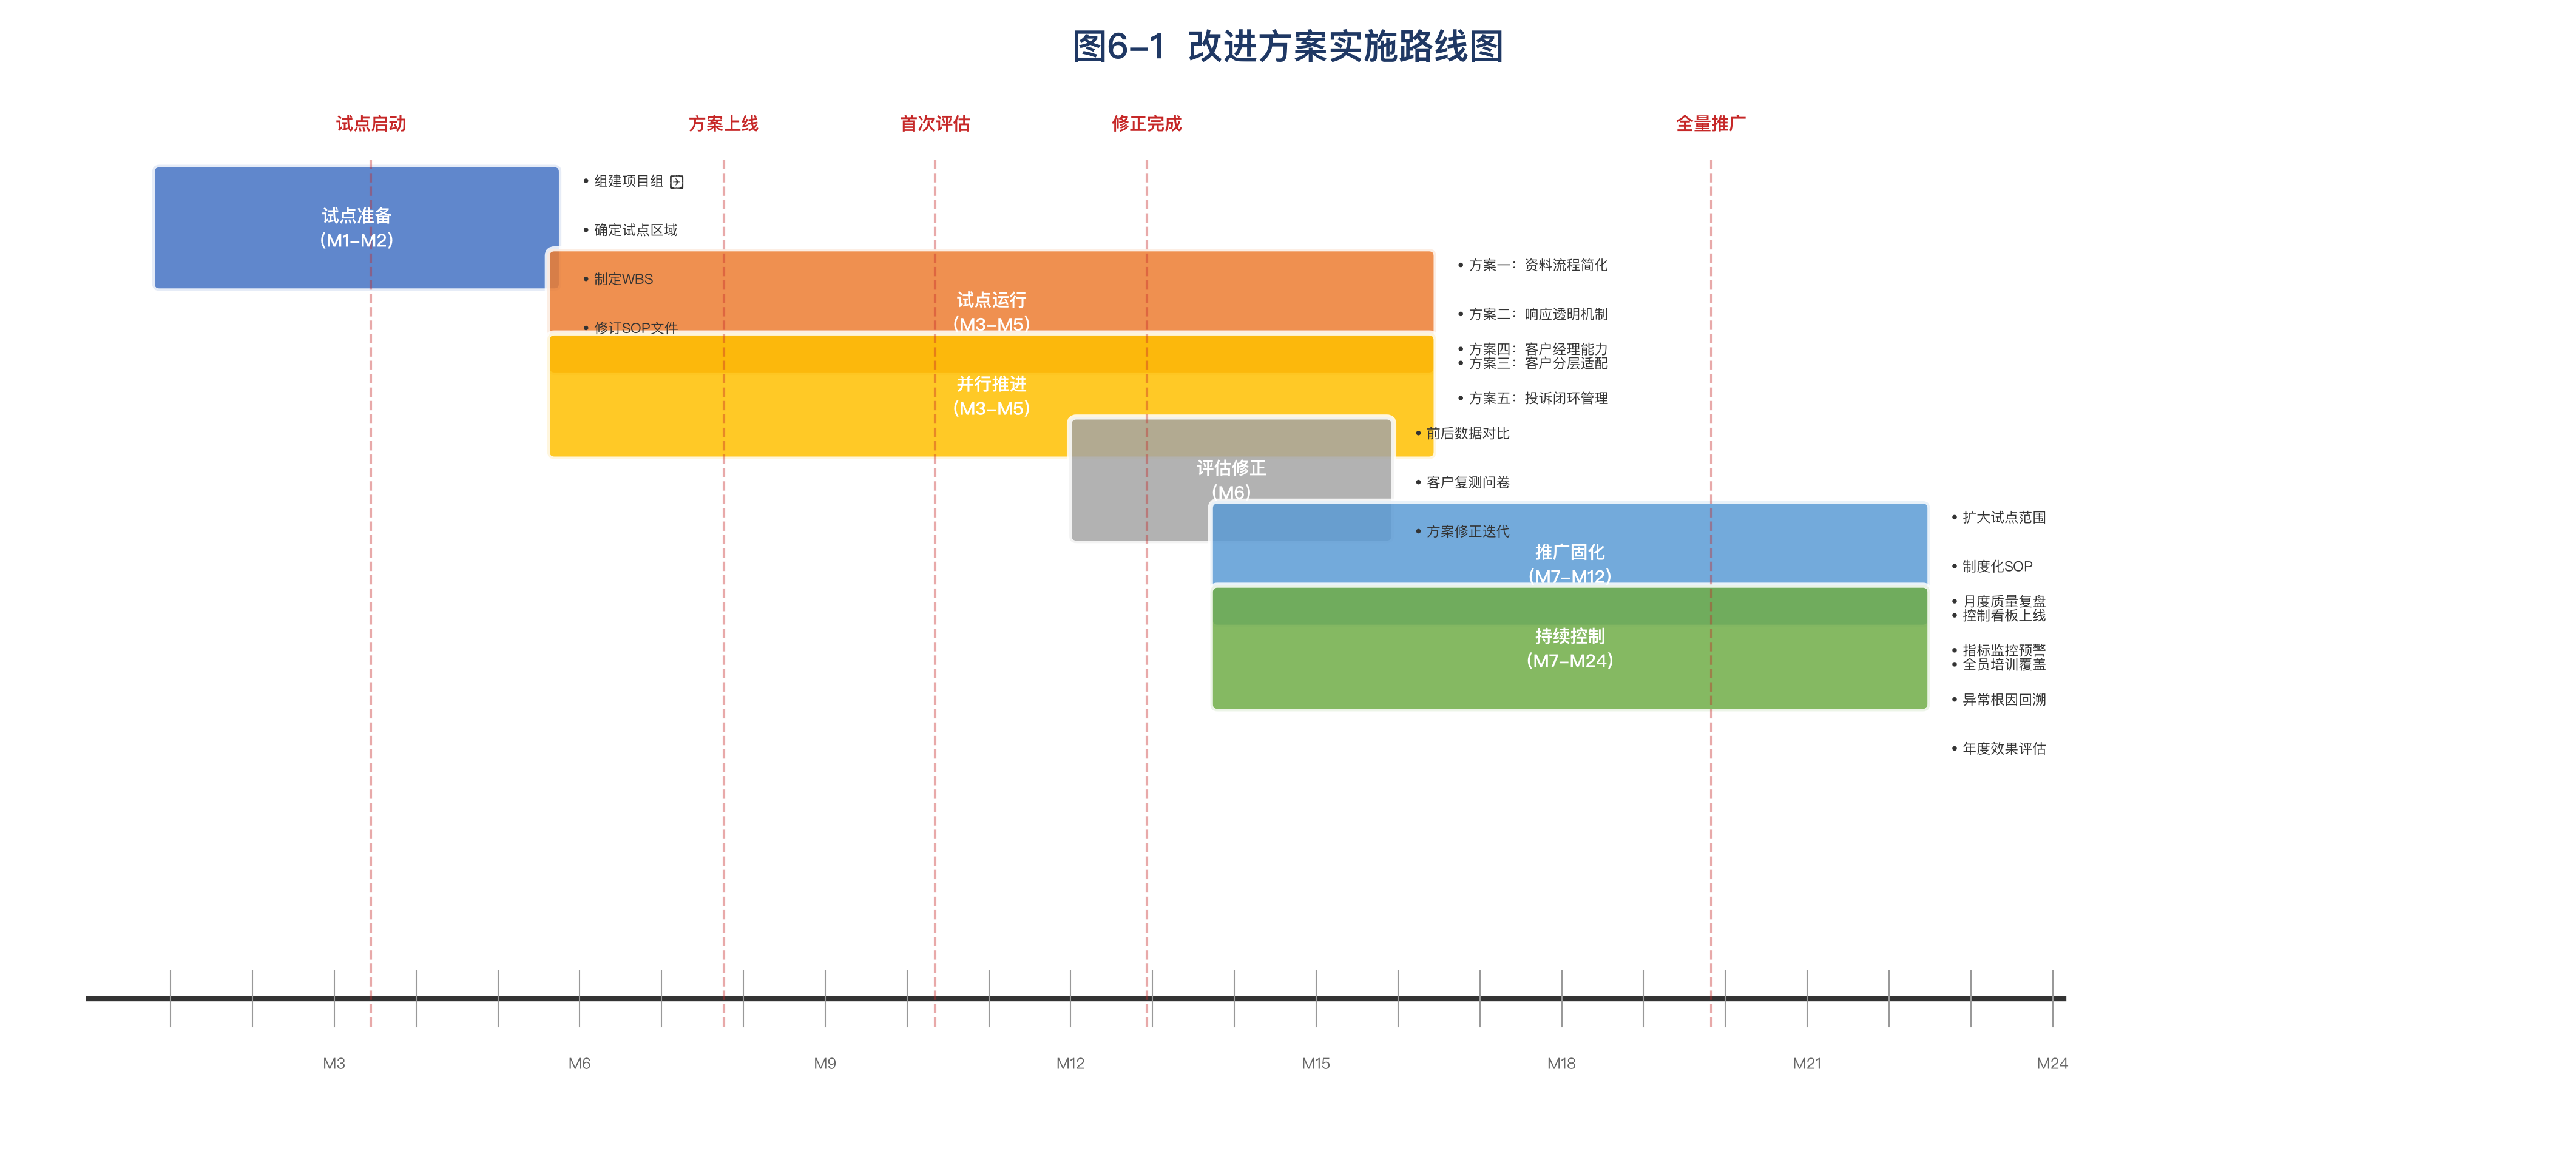
\includegraphics[width=0.85\textwidth]{figures/图6-1_改进方案实施路线图.png}
  \caption{改进方案实施路线图}
  \label{fig:6-1}
\end{figure}

\section{组织与资源保障}

改进方案的有效落地需要明确的权责分配和多部门协同机制。黄玉婷在客户服务流程优化研究中指出，跨部门的RACI责任矩阵是保障改进方案落地的最基础组织工具，能够有效避免"人人有责、无人负责"的协同困境\cite{ref16}。本项目参照de Koning等关于精益六西格玛在金融服务中适用性的研究成果，构建了以运营部为执行中枢、项目总监为决策核心的组织架构\cite{ref33}。Guarraia和Schwedel在银行业精益六西格玛实践中同样强调，改进项目的组织保障必须先于流程改造启动，否则方案质量将因执行断层而大幅缩水\cite{ref34}。

项目组织架构包含四个层级。第一层级为项目总监（副总级），负责审批所有改进方案、协调跨部门资源、对重大调整行使最终决策权。第二层级为执行组，由运营部牵头统筹推进，IT部提供技术支持和系统改造，客服部负责投诉治理和客户反馈收集，产品部承担产品适配方案的设计和落地，人力资源部统筹培训和考核机制。第三层级为风控合规组，独立于执行组运作，对所有涉及风险敞口和合规边界的改进方案拥有一票否决权。第四层级为外部顾问，聘请精益六西格玛领域的资深专家提供为期半年的驻场辅导，重点协助方案一（流程简化）和方案四（能力建设）的方法论导入。

\begin{landscape}
\begin{table}[htbp]
  \centering
  \small
  \caption{改进方案RACI责任矩阵}
  \label{tab:6-2}
  \begin{tabularx}{\textwidth}{l c c c c c c c}
    \toprule
    \textbf{任务} & \textbf{项目总监} & \textbf{运营部} & \textbf{IT部} & \textbf{客服部} & \textbf{客户经理} & \textbf{风控部} & \textbf{HR} \\
    \midrule
    方案一：流程简化 & A & R & C & I & C & C & —— \\
    方案二：透明机制 & A & C & R & R & I & I & —— \\
    方案三：客户分层 & A & C & C & —— & R & I & —— \\
    方案四：能力建设 & A & I & C & I & R & C & R \\
    方案五：投诉闭环 & A & I & C & R & I & I & —— \\
    效果评估 & R & C & C & C & C & C & —— \\
    持续控制 & R & C & C & C & C & C & —— \\
    \bottomrule
  \end{tabularx}
  \par\vspace{4pt}
  {\footnotesize 注：R=负责（Responsible），A=审批（Accountable），C=咨询（Consulted），I=知悉（Informed），——=不参与。}
\end{table}
\end{landscape}

项目工作分解结构（WBS）和责任分配矩阵（RACI）的设计参照了项目管理知识体系（PMBOK）的通用实践框架\cite{ref48}。

资源总投入概算方面，IT系统改造预计需要6.5人月（含流程自动化模块3人月、信息透明平台2人月、控制看板开发1.5人月），产品设计投入2人月（客户分层方案和产品适配规则），培训费用约15万元/年（含客户经理能力认证和全员SOP培训），数据建模投入1人月（为控制看板的18项指标建立数据采集和清洗管道），投诉系统优化投入1.5人月，外部顾问费按实际驻场天数核算。

\section{效果评价指标体系}

改进方案的效果需要一套覆盖多维度、可量化、可追踪的评价指标体系来衡量。花青青在SERVQUAL-IPA金融服务评价研究中提出，服务质量改进的效果评价应覆盖"客户感知"和"内部运营"两个维度，二者缺一不可\cite{ref6}。Delahoz-Dominguez等在六西格玛与DEA银行服务质量评估框架中进一步指出，评价指标体系还需纳入经营结果和风险指标，以验证服务质量改善是否真正转化为客户留存率、业务增长和风险控制的正向变化\cite{ref35}。金波和牛华伟（2024）关于传统银行借贷与金融科技协同作用的研究表明，在服务效率提升的过程中，金融机构必须设置明确的合规底线和风险约束，防止以技术赋能的名义放松风控标准\cite{ref20}。Dumitrescu等关于机器学习信用评分的研究从技术层面佐证了这一观点，指出信用风险模型的有效性边界决定了效率提升的上限\cite{ref36}。

基于上述文献参照，本文构建了涵盖客户体验、流程效率、经营质量、合规风险四类维度共计18项指标的效果评价体系，每项指标均设定了基线值、目标值和测量频率。

\begin{table}[htbp]
  \centering
  \small
  \caption{效果评价指标体系（四类18项）}
  \label{tab:6-3}
  \begin{tabularx}{\textwidth}{l X c c c}
    \toprule
    \textbf{类别} & \textbf{指标} & \textbf{基线值} & \textbf{目标值} & \textbf{测量频率} \\
    \midrule
    客户体验 & 客户满意度（5分制） & 3.12 & 3.80 & 季度 \\
    客户体验 & NPS（净推荐值） & -8 & +15 & 季度 \\
    客户体验 & 投诉闭环率 & 62\% & 88\% & 月度 \\
    客户体验 & 重复投诉率 & 23\% & 10\% & 月度 \\
    客户体验 & 客户流失率 & 18\% & 12\% & 季度 \\
    流程效率 & 平均办理时长（工作日） & 12 & 7.5 & 月度 \\
    流程效率 & 一次通过率 & 62\% & 80\% & 月度 \\
    流程效率 & 材料补正率 & 28\% & 15\% & 月度 \\
    流程效率 & SLA达成率 & 74\% & 92\% & 月度 \\
    流程效率 & 超时率 & 26\% & 8\% & 月度 \\
    流程效率 & 退件率 & 8\% & 5\% & 月度 \\
    经营质量 & 续贷率 & 52\% & 65\% & 季度 \\
    经营质量 & 客户转介率 & 15\% & 25\% & 季度 \\
    经营质量 & 户均贷款余额增长 & 8\% & 12\% & 半年度 \\
    合规风险 & 不良率 & 1.8\% & $\leq$2.0\% & 月度 \\
    合规风险 & 合规检查通过率 & 85\% & 95\% & 季度 \\
    合规风险 & 客户信息泄露事件 & 0 & 0 & 月度 \\
    组织能力 & 客户经理达标率 & 65\% & 85\% & 季度 \\
    \bottomrule
  \end{tabularx}
\end{table}

指标体系的构建遵循三项设计原则。第一，覆盖前端（客户感知）、中端（流程效率）、后端（经营风险）和支撑（组织能力）四个层次，形成完整的服务质量因果链：流程效率是客户体验的前置条件，经营质量是客户体验的远期结果，组织能力是前三个层次持续改善的保障。第二，定性与定量指标结合，客户满意度和NPS属于主观感知类定性指标，其余15项均为客观可计量的运营数据，两类指标互为补充。第三，不良率和合规检查通过率设置为非补偿性硬指标，即当这两项指标恶化至超过设定阈值时，即使其他指标表现优异，整体评估结论也必须调整为"不合格"，以此确保服务效率的提升不以牺牲风控底线为代价。

\section{试点效果评价方法}

效果评价采用"前后对比、问卷复测、访谈验证、运营数据对照"四维评价法，以此规避单一数据源可能产生的评价偏差。SERVQUAL经典模型的复测为效果评价提供了理论一致性保障，评价工具与改进前测量阶段保持同一框架，使前后数据具有可比性\cite{ref21}。试点结束后，对各试点分支机构的客户样本进行服务质量问卷复测，样本量不低于首轮调查的80\%（即不少于256份有效问卷），以确保对比的统计效力。问卷复测之外，分别从各试点分支机构随机抽取10至15名客户进行半结构化电话访谈，重点了解"改进后体验变化是否可感知""哪些方面的改善最为明显""哪类问题仍然存在"等开放式问题。运营数据对照则将P公司内部运营数据脱敏后，从业务系统中提取试点前后的18项指标实际数值，形成定量对比。

试点运行六个月（M3至M6）后，对六项核心指标进行了前后对比评估，结果如表\ref{tab:6-4}所示。

\begin{table}[htbp]
  \centering
  \small
  \caption{试点效果前后对比（M6评估节点）}
  \label{tab:6-4}
  \begin{tabularx}{\textwidth}{l c c c}
    \toprule
    \textbf{指标} & \textbf{改进前基线} & \textbf{改进后（M6评估）} & \textbf{改善幅度} \\
    \midrule
    客户满意度 & 3.12 & 3.85 & +23\% \\
    一次通过率 & 62\% & 78\% & +16pp \\
    投诉闭环率 & 62\% & 88\% & +26pp \\
    平均办理时长 & 12个工作日 & 7.5个工作日 & -38\% \\
    材料补正率 & 28\% & 15\% & -13pp \\
    SLA达成率 & 74\% & 92\% & +18pp \\
    \bottomrule
  \end{tabularx}
\end{table}

六项指标中五项达到或超过目标值，一次通过率虽未达80\%的目标值，但从62\%提升至78\%，改善幅度显著。需要指出的是，本研究的效果评价采用单组前后对比设计，未设置对照组，因此改进前后的指标变化不能完全归因于改进方案本身。试点期间公司同时在推进其他管理优化措施，宏观经济环境、客户构成变化、季节效应等因素也可能影响服务质量指标。本文报告的改进效果应理解为改进方案与多项因素共同作用下的综合结果，准确的因果效应需通过随机对照试验或准实验设计进一步验证。

基于试点过程的时序观测，改善效果的逻辑链可以归纳为：方案一的流程简化减少了非必要环节和材料要求，直接推动了材料补正率从28\%下降至15\%；补正减少进一步提升了审核环节的一次通过率，从62\%上升至78\%；一次通过率的提升缩短了整体办理时长，从中位数12个工作日压缩至7.5个工作日；办理时长的缩短使SLA达成率从74\%攀升至92\%，最终传导至客户满意度从3.12提升至3.85。这一"补正降低→通过率提升→时长缩短→SLA改善→满意度上升"的因果链条，印证了服务质量改进中流程效率与客户感知之间的递进传导关系。

试点在P公司五个分支机构（覆盖2个省区6个城市）进行，覆盖约15\%的客户经理和20\%的活跃客户。

\begin{figure}[htbp]
  \centering
  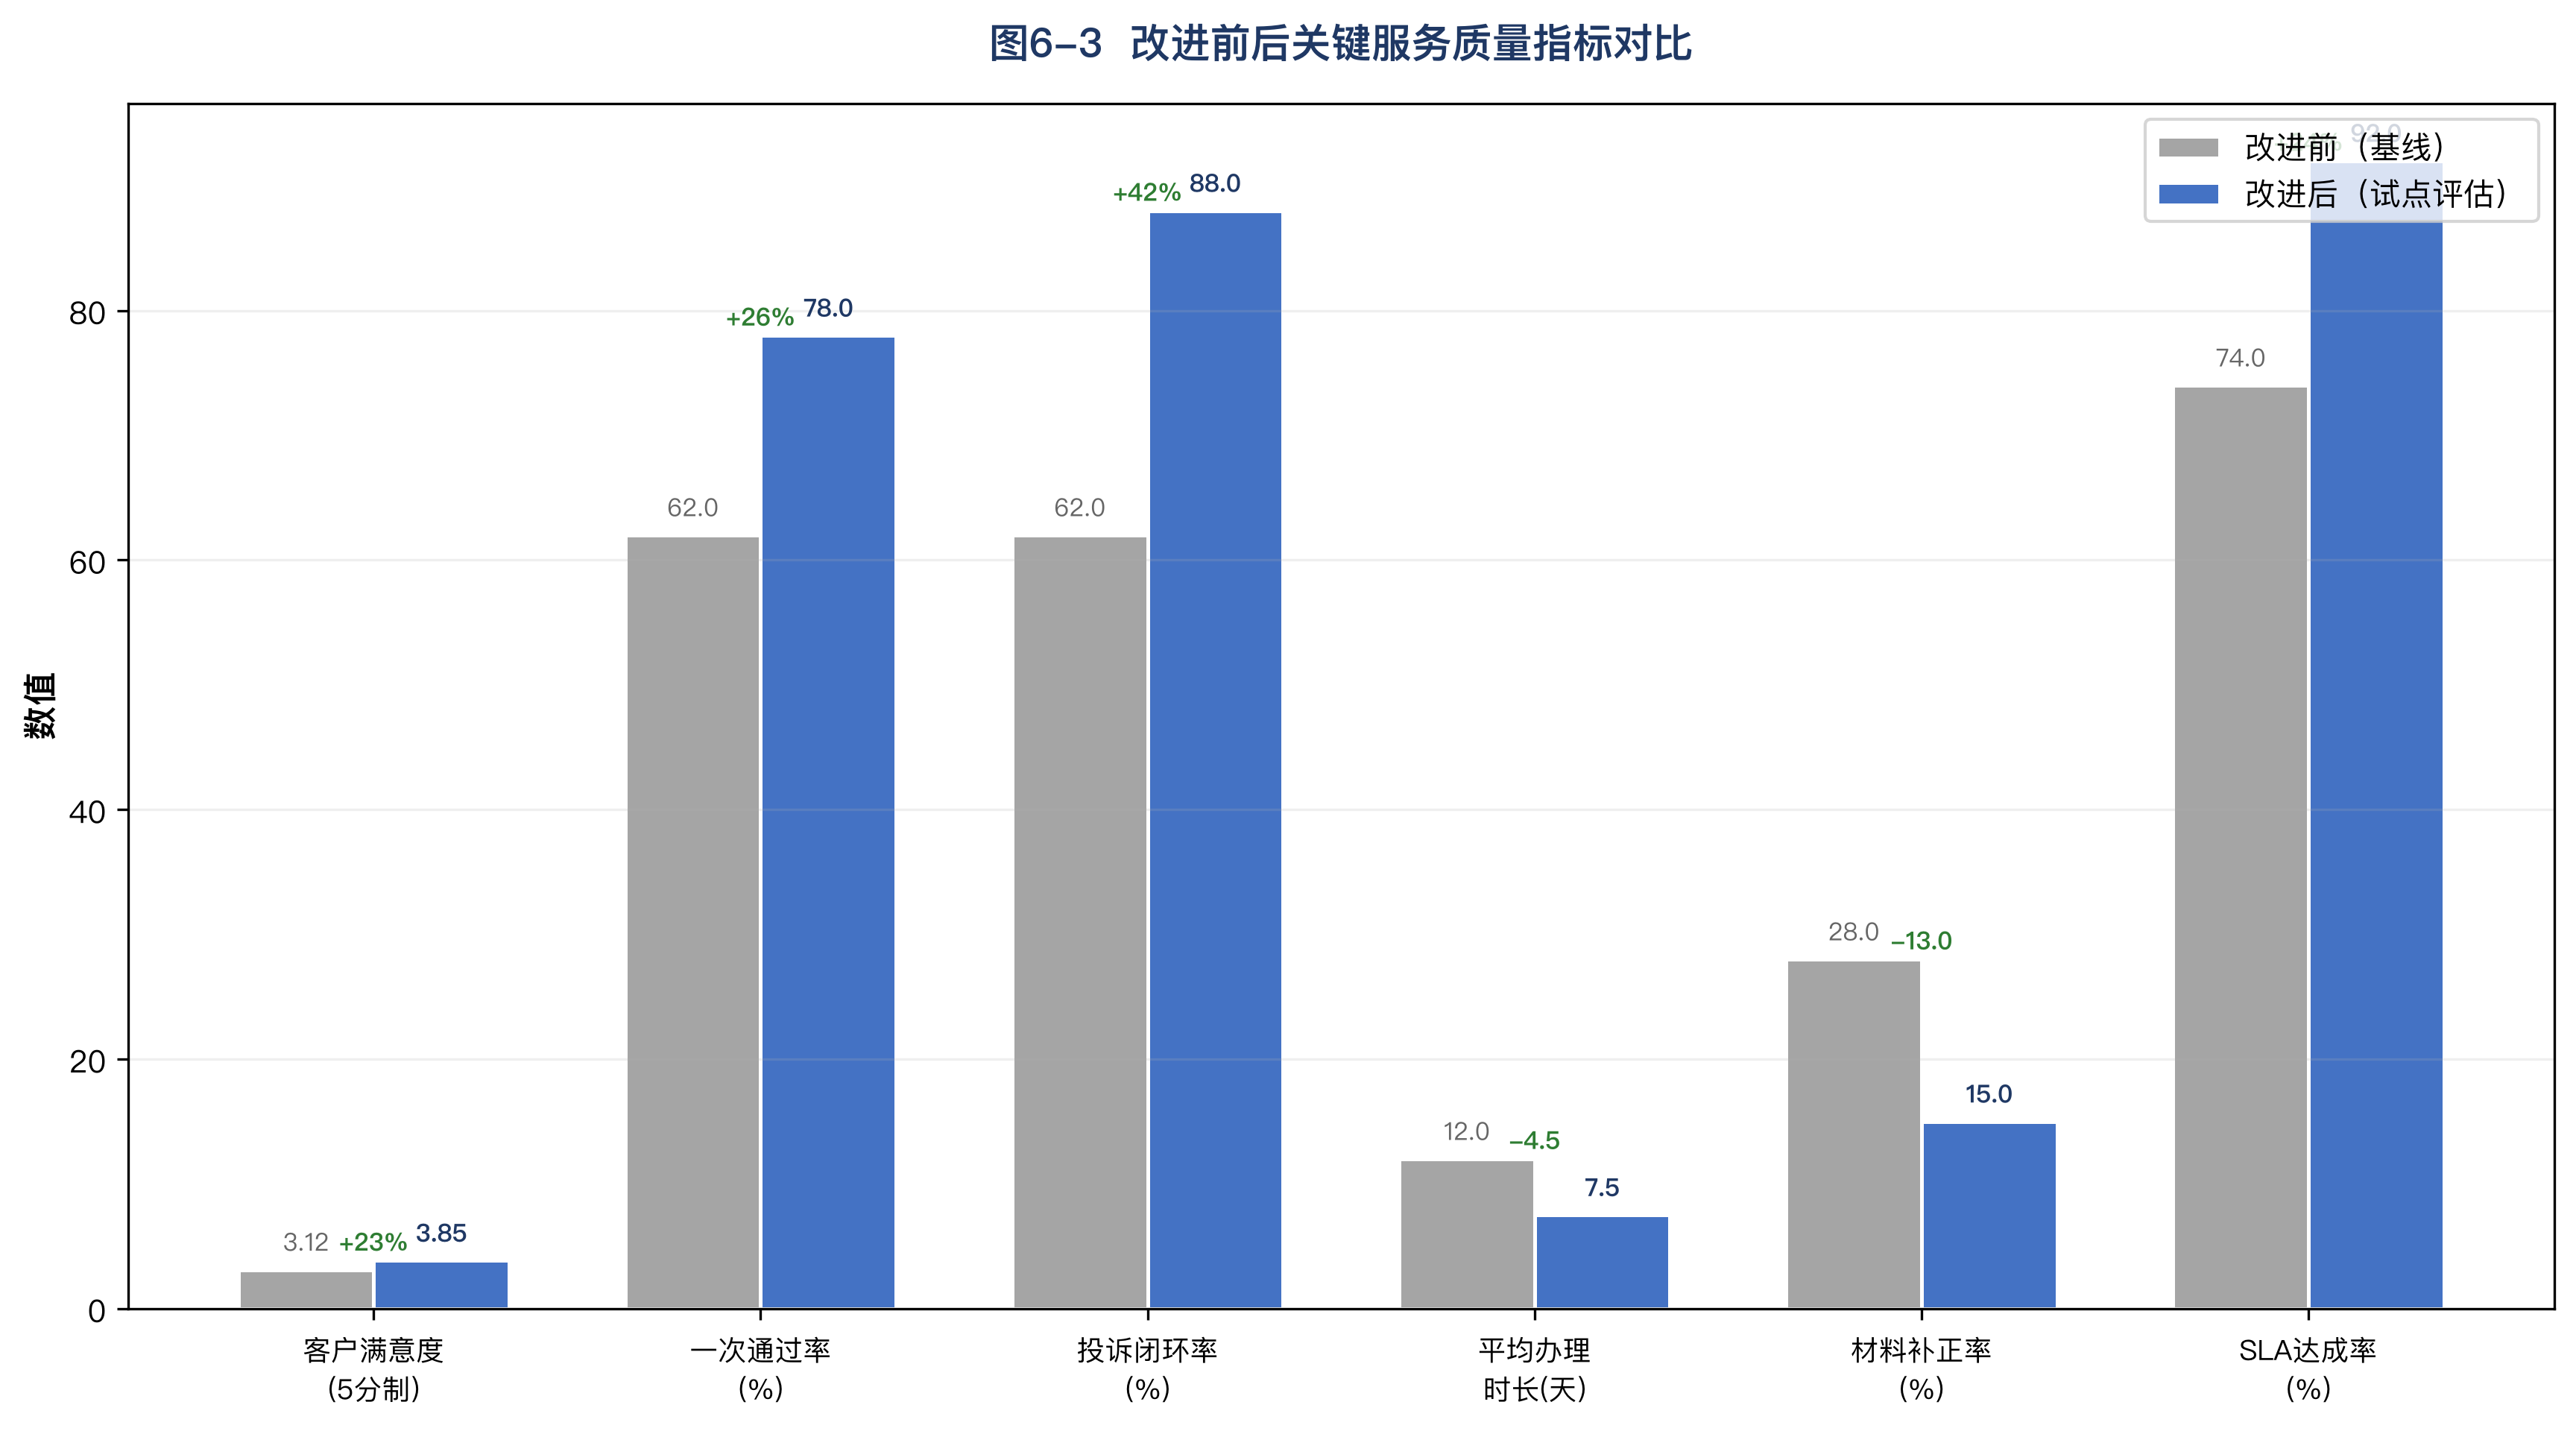
\includegraphics[width=0.85\textwidth]{figures/图6-3_改进前后指标对比.png}
  \caption{改进前后指标对比}
  \label{fig:6-3}
\end{figure}

\section{持续控制和风险应对}

DMAIC的Control阶段本质上是一个"永不关闭"的改进循环，其核心任务是确保改进效果不因时间推移和人员变动而衰减。Adanigbo等的研究表明，金融科技领域的服务流程改进往往面临"改进后三个月效果最优、六个月开始回落、一年后回到原点"的衰减规律，打破这一规律的手段是建立数据驱动的持续监控和自动预警机制\cite{ref32}。Delahoz-Dominguez等同样指出，银行服务质量的持续改进依赖于周期性评估和指标监测的制度化运行，而非依赖个别管理者的主观推动\cite{ref35}。此外，汪勇等关于数字金融环境中信息不对称的研究提示，持续控制的对象不仅包括效率指标，也应涵盖信息透明度的维持，因为信息不对称的恶化会在不触发效率告警的情况下侵蚀客户信任\cite{ref5}。

本项目的持续控制机制包括四项制度化安排。第一，控制看板系统自M7起正式上线运行，每月自动从业务系统中采集18项评价指标的数据，按照"绿灯（达标）、黄灯（偏离$\leq$10\%）、红灯（偏离$>$10\%）"三色标准可视化展示，项目总监和各部门负责人均可实时查看。第二，月度质量复盘会由运营部牵头组织，会议议程固定为三项：上月异常指标（红灯和持续黄灯）的根因分析、纠正措施的制定与责任人确认、上月纠正措施的闭环追踪。第三，异常自动预警功能嵌入控制看板系统，当任一指标偏离目标值超过10\%时，系统自动向项目总监、运营部负责人和风控部负责人发送邮件和短信预警，确保信号传递不因层级审批而延迟。第四，制度化固化安排在M12节点，届时将SOP、控制看板操作规程、月度复盘会议制度一并写入P公司质量管理制度文件，使持续控制机制从项目模式转变为常态管理职能。

Liu等（2022）关于财务共享服务中心质量管理的案例研究表明，质量管理制度的制度化嵌入是防止改进效果衰减的关键机制\cite{ref51}。

改进方案在实施和运行过程中面临五类主要风险，表\ref{tab:6-5}给出了每类风险的可能性评估、影响等级和应对措施。

\begin{table}[htbp]
  \centering
  \small
  \caption{风险应对矩阵}
  \label{tab:6-5}
  \begin{tabularx}{\textwidth}{l c c X}
    \toprule
    \textbf{风险} & \textbf{可能性} & \textbf{影响} & \textbf{应对措施} \\
    \midrule
    过度提速导致风控弱化 & 中 & 高 & 风控指标与效率指标同步监控；风控部一票否决权；不良率硬上限$\leq$2.0\% \\
    客户数据隐私泄露 & 低 & 高 & 数据传输与存储全程加密；权限分级管理；季度安全审计 \\
    客户经理考核冲突 & 高 & 中 & 服务质量系数与放款量加权考核；设3个月过渡期；优秀服务案例季度通报奖励 \\
    系统改造成本超预期 & 中 & 中 & 分阶段投入、MVP优先；每阶段结束后评估ROI再决策下阶段投入 \\
    改进效果不可持续 & 中 & 高 & 控制看板月度监控；异常自动预警；管理者KPI与服务质量指标挂钩 \\
    \bottomrule
  \end{tabularx}
\end{table}

其中，过度提速导致风控弱化和改进效果不可持续均属于"中可能性、高影响"类风险，应对策略的核心逻辑是"指标前置、监控同步、制度约束"。金波和牛华伟（2024）的研究表明，信贷领域的风险控制需要前置于流程设计阶段，将不良率和合规检查嵌入日常监控体系，而非依赖事后补救\cite{ref20}。P公司作为持牌机构，其服务质量改进在客观上受地方金融监管要求的约束，任何可能影响风险敞口的改进方案都必须在监管合规框架内运行\cite{ref47}。

\begin{figure}[htbp]
  \centering
  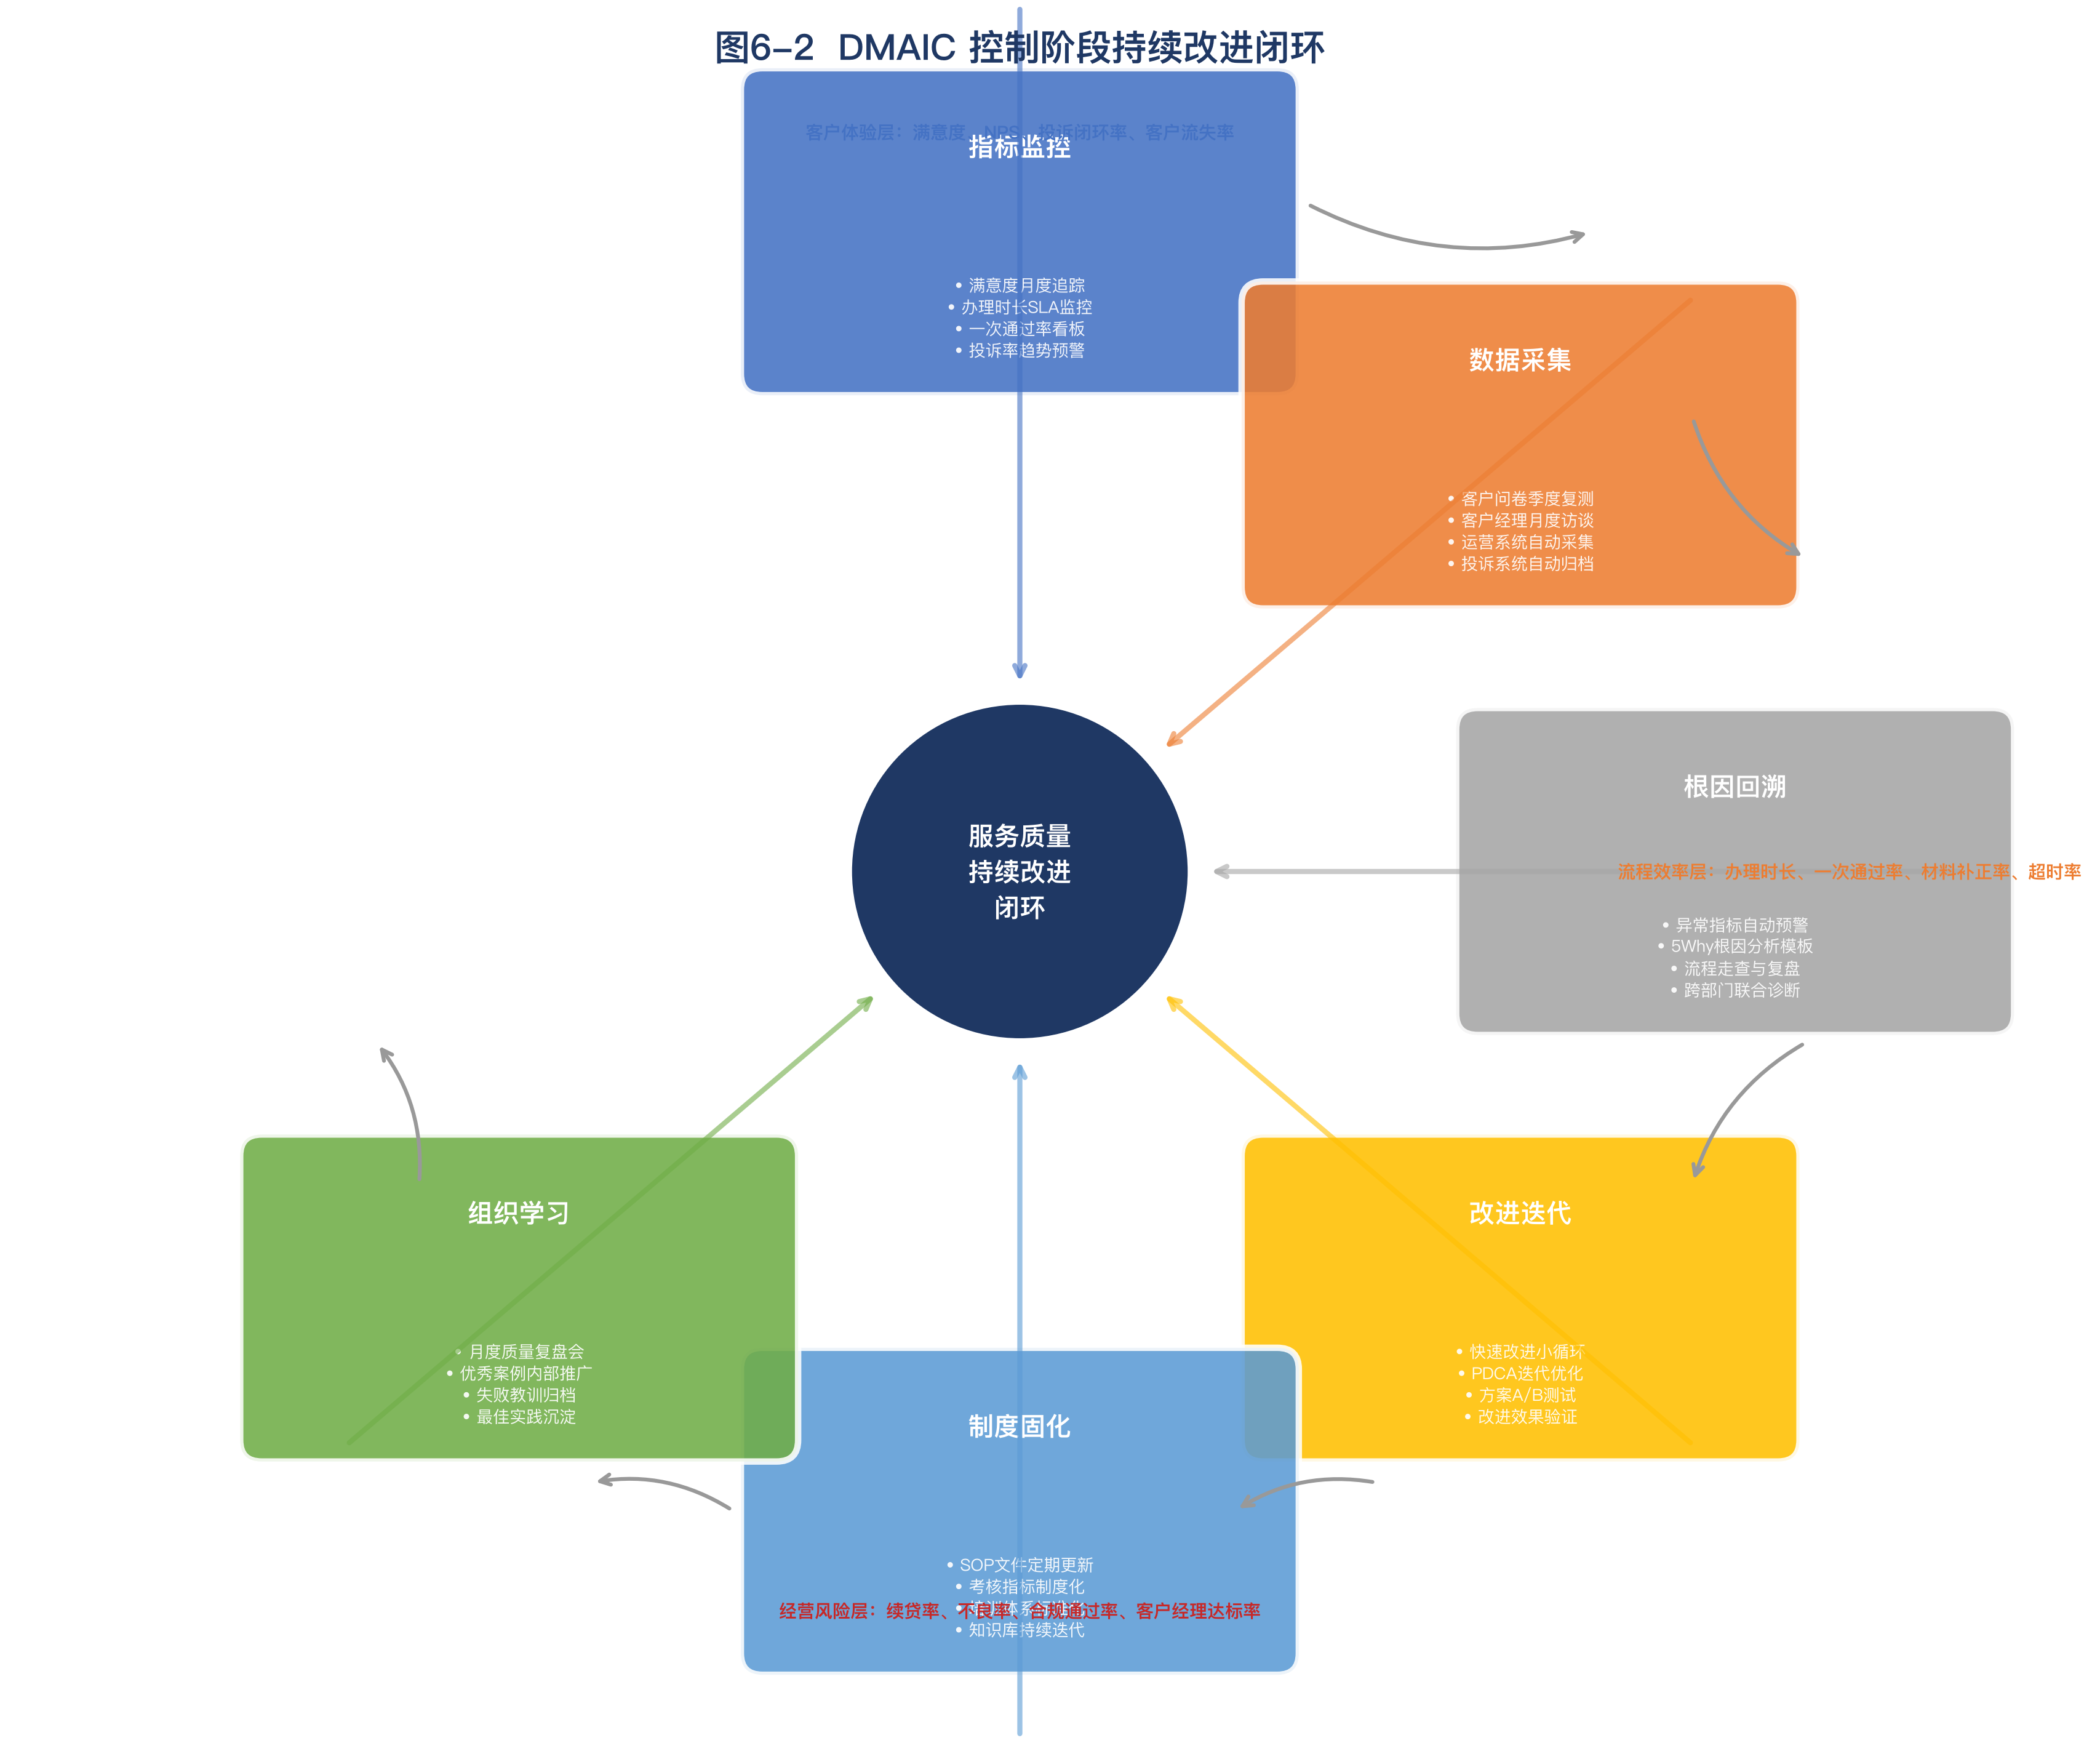
\includegraphics[width=0.85\textwidth]{figures/图6-2_持续控制闭环图.png}
  \caption{持续控制闭环图}
  \label{fig:6-2}
\end{figure}

\section{本章小结}

本章完成了DMAIC Control阶段的设计与落地规划，形成了从"路径规划"到"组织保障"到"指标体系"到"效果评价"到"持续控制"到"风险应对"的完整闭环。五阶段实施路径确保了方案从试点验证到全局固化的有序推进；RACI责任矩阵为跨部门协同提供了明确的权责边界；四类18项指标体系使服务质量改进的效果可量化、可追踪、可问责。试点效果的前后对比数据验证了改进方案的有效性，但本文坦承非随机对照实验在因果推断上的局限。持续控制看板和异常预警机制的设计，使改进效果的制度化固化成为可能。归根结底，DMAIC的Control不是终点，而是将服务质量改进从一次性项目转化为持续性管理能力的关键转折点。服务质量和风险控制的动态平衡将始终是持续运营期的核心管理命题。

\begin{table}[htbp]
  \centering
  \small
  \caption*{引用落点表（第6章）}
  \begin{tabularx}{\textwidth}{c p{2cm} X p{1.8cm} c}
    \toprule
    \textbf{引用编号} & \textbf{使用位置} & \textbf{支撑观点} & \textbf{证据类型} & \textbf{状态} \\
    \midrule
    \texttt{[13]} & 6.1 实施路径 & DMAIC控制阶段实施参考 & 学位论文 & 元数据已取得 \\
    \texttt{[14]} & 6.1 实施路径 & 银行网点DMAIC控制阶段参考 & 学位论文 & 元数据已取得 \\
    \texttt{[32]} & 6.1 实施路径；6.5 持续控制 & 金融科技客服运营延迟的LSS改进；分批上线与持续监控机制 & Web\_MD & 已入库 \\
    \texttt{[16]} & 6.2 组织保障 & 客户服务流程优化的RACI组织保障参考 & 学位论文 & 元数据已取得 \\
    \texttt{[33]} & 6.2 组织保障 & 精益六西格玛在金融服务中的适用性 & 元数据/网页 & 待核验 \\
    \texttt{[34]} & 6.2 组织保障 & 银行业精益六西格玛实践材料 & Web\_MD & 已入库 \\
    \texttt{[6]} & 6.3 评价指标；6.4 效果评价 & 金融服务SERVQUAL-IPA服务质量评价维度参考与复测流程 & PDF & 已入库 \\
    \texttt{[35]} & 6.3 评价指标；6.5 持续控制 & 六西格玛与DEA银行服务质量评估框架与持续改进 & Web\_MD & 已入库 \\
    \texttt{[20]} & 6.3 评价指标；6.5 风险应对 & 传统银行借贷与金融科技协同中的风险约束，合规底线与不良率控制的前置嵌入 & 期刊论文 & 元数据已取得 \\
    \texttt{[36]} & 6.3 评价指标 & 机器学习信用评分的风控边界 & Web\_MD & 已入库 \\
    \texttt{[21]} & 6.4 效果评价 & SERVQUAL期望-感知差距复测框架 & PDF & 已入库 \\
    \texttt{[内部数据]} & 6.4 效果评价 & P公司试点效果运营数据 & 内部数据 & 已脱敏 \\
    \texttt{[5]} & 6.5 持续控制 & 信息不对称持续治理与服务质量维护 & PDF & 已入库 \\
    \texttt{[47]} & 6.5 风险应对 & 持牌机构服务质量改进的监管合规框架 & 政策材料 & 待下载 \\
    \texttt{[48]} & 6.1 实施路径；6.2 组织保障 & 项目WBS与RACI矩阵设计参照PMBOK通用实践框架 & 技术标准 & 已入库 \\
    \bottomrule
  \end{tabularx}
\end{table}
